% !TeX encoding = UTF-8
% !TeX spellcheck = en_GB
% !TeX root = mythesis.tex
\chapter{Wigner function of different charge per pulse}

%The  Forth appendix

\section{A non integer charge Lorentzian pulse}

\subsection{Wigner}

\begin{figure}[hpbt]
	\centering
	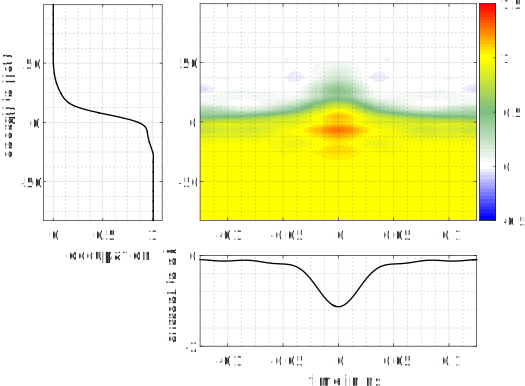
\includegraphics[width = 10cm]{./appD/wigData_leviton_20ps_0_5e_51mK_Projected_Gradient_Method}
	\caption{wigner du 0.5e 25ps}
	\label{fig: wigner du 0.5e 20ps}
\end{figure}

\subsection{Probabilities and Coherences}

\begin{figure}[hptb]
	\begin{center}
		\begin{tabular}{c c c c}
			(a) & & &   \\ 
			& 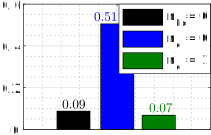
\includegraphics[width = 5cm]{./appD/JnlData_leviton_20ps_0_5e_51mK_Projected_Gradient_Method_proba} &
			&  \\
			(b) & & (c) & \\
			& 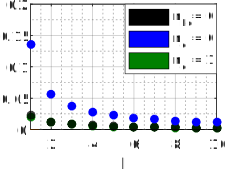
\includegraphics[width = 5cm]{./appD/JnlData_leviton_20ps_0_5e_51mK_Projected_Gradient_Method_coh_inter_period} &
			& 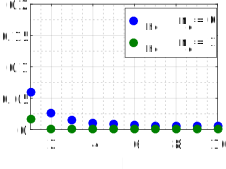
\includegraphics[width = 5cm]{./appD/JnlData_leviton_20ps_0_5e_51mK_Projected_Gradient_Method_coh_el_ho}
		\end{tabular} 
	\end{center}
	\caption{(a) pi du 0.5e 20ps (b) coh du 0.5e 20ps}
	\label{fig: Jnl du 0.5e 20ps}
\end{figure}

\subsection{Wavefunctions}

\begin{figure}[hptb]
	\begin{center}
		\begin{tabular}{c c c c}
			
			(a) & & (b) &  \\ 
			& 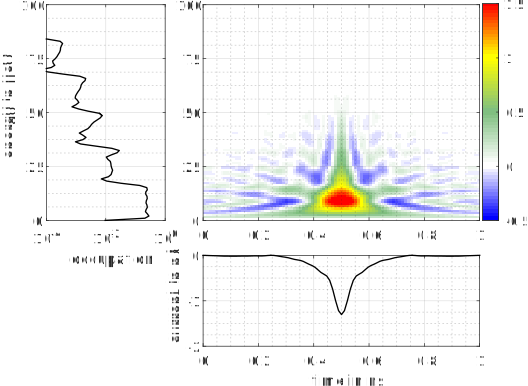
\includegraphics[width = 6.5 cm]{./appD/wannierwigData_leviton_20ps_0_5e_51mK_Projected_Gradient_Method-el-0} &
			& \includegraphics[width = 6.5 cm]{./appD/wannierwigData_leviton_20ps_0_5e_51mK_Projected_Gradient_Method-el-1} \\
			(c) & & & \\
			& 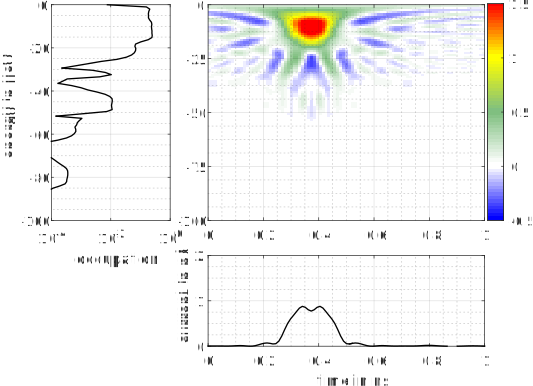
\includegraphics[width = 6.5 cm]{./appD/wannierwigData_leviton_20ps_0_5e_51mK_Projected_Gradient_Method-ho-0} & &
		\end{tabular} 
	\end{center}
	\caption{(a) wannier el-0 du 0.5e 25ps overlap de 0.98 avec leviton \underline{50 ps} (b) wannier el-1 du 0.5e 20ps (c) wannier ho-0 du 0.5e 20ps}
	\label{fig: wannier du 0.5e 20ps}
\end{figure}

\section{An analysis for different charge electron than holes periodic pulses}

